% Created 2020-07-07 mar. 18:24
% Intended LaTeX compiler: pdflatex
\documentclass{ISMA_USD2020}
\usepackage[utf8]{inputenc}
\usepackage[T1]{fontenc}
\usepackage{graphicx}
\usepackage{grffile}
\usepackage{longtable}
\usepackage{wrapfig}
\usepackage{rotating}
\usepackage[normalem]{ulem}
\usepackage{amsmath}
\usepackage{textcomp}
\usepackage{amssymb}
\usepackage{capt-of}
\usepackage{hyperref}
\usepackage[most]{tcolorbox}
\usepackage{bm}
\usepackage{booktabs}
\usepackage{tabularx}
\usepackage{array}
\usepackage{siunitx}
\usepackage{amsmath,amssymb,amsfonts, cases}
\usepackage{algorithmic, graphicx, textcomp}
\usepackage{xcolor, import, hyperref}
\usepackage{subcaption}
\usepackage[USenglish, english]{babel}
\setcounter{footnote}{1}
\input{config.tex}
\author[1,3] {T. Dehaeze}
\author[1,2] {C. Collette}
\affil[1] {Precision Mechatronics Laboratory\NewLineAffil University of Liege, Belgium \NewAffil}
\affil[2] {BEAMS Department\NewLineAffil Free University of Brussels, Belgium \NewAffil}
\affil[3] {European Synchrotron Radiation Facility \NewLineAffil Grenoble, France e-mail: \textbf{thomas.dehaeze@esrf.fr}}
\bibliographystyle{IEEEtran}
\usepackage{tikz}
\usetikzlibrary{shapes.misc,arrows,arrows.meta}
\date{}
\title{Active Damping of Rotating Platforms using Integral Force Feedback}
\hypersetup{
 pdfauthor={},
 pdftitle={Active Damping of Rotating Platforms using Integral Force Feedback},
 pdfkeywords={},
 pdfsubject={},
 pdfcreator={Emacs 27.0.91 (Org mode 9.4)}, 
 pdflang={English}}
\begin{document}

\maketitle

\abstract{
This paper investigates the use of Integral Force Feedback (IFF) for the active damping of rotating mechanical systems.
Guaranteed stability, typical benefit of IFF, is lost as soon as the system is rotating due to gyroscopic effects.
To overcome this issue, two modifications of the classical IFF control are proposed.
The first consists of slightly modifying the control law while the second consists of adding springs in parallel with the force sensors.
Conditions for stability and optimal parameters are derived.
The results reveal that, despite their different implementations, both modified IFF control have almost identical damping authority on suspension modes.
}

\section{Introduction}
\label{sec:org72e892d}
\label{sec:introduction}
There is an increasing need to reduce the undesirable vibration of many sensitive equipment.
A common method to reduce vibration is to mount the sensitive equipment on a suspended platform which attenuates the vibrations above the frequency of the suspension modes.
In order to further decrease the residual vibrations, active damping can be used for reducing the magnification of the response in the vicinity of the resonances.

In \cite{preumont92_activ_dampin_by_local_force}, the Integral Force Feedback (IFF) control scheme has been proposed, where a force sensor, a force actuator and an integral controller are used to directly augment the damping of a mechanical system.
When the force sensor is collocated with the actuator, the open-loop transfer function has alternating poles and zeros which facilitate to guarantee the stability of the closed loop system \cite{preumont02_force_feedb_versus_accel_feedb}.

However, when the platform is rotating, the system dynamics is altered and IFF cannot be applied as is.
The purpose of this paper is to study how the IFF strategy can be adapted to deal with these Gyroscopic effects.

The paper is structured as follows.
Section \ref{sec:dynamics} presents a simple model of a rotating suspended platform that will be used throughout this study.
Section \ref{sec:iff} explains how the unconditional stability of IFF is lost due to Gyroscopic effects induced by the rotation.
Section \ref{sec:iff_hpf} suggests a simple modification of the control law such that damping can be added to the suspension modes in a robust way.
Section \ref{sec:iff_kp} proposes to add springs in parallel with the force sensors to regain the unconditional stability of IFF.
Section \ref{sec:comparison} compares both proposed modifications to the classical IFF in terms of damping authority and closed-loop system behavior.

\section{Dynamics of Rotating Positioning Platforms}
\label{sec:org967f3ca}
\label{sec:dynamics}
In order to study how the rotation of a positioning platforms does affect the use of integral force feedback, a model of an XY positioning stage on top of a rotating stage is used.
Figure \ref{fig:system} represents the model schematically.
This model is the simplest in which gyroscopic forces can be studied.

\begin{figure}[htbp]
\centering
\includegraphics[scale=1]{figs/system.pdf}
\caption{\label{fig:system}Schematic of the studied System}
\end{figure}

The rotating stage is supposed to be ideal, meaning it induces a perfect rotation \(\theta(t) = \Omega t\) where \(\Omega\) is the rotational speed in \(\si{\radian\per\second}\).

The parallel XY positioning stage consists of two orthogonal actuators represented by three elements in parallel: a spring with a stiffness \(k\) in \(\si{\newton\per\meter}\), a dashpot with a damping coefficient \(c\) in \(\si{\newton\per\meter\second}\) and an ideal force source \(F_u, F_v\).
A payload with a mass \(m\) in \(\si{\kilo\gram}\) is mounted on the (rotating) XY stage.

Two reference frames are used: an inertial frame \((\vec{i}_x, \vec{i}_y, \vec{i}_z)\) and a uniform rotating frame \((\vec{i}_u, \vec{i}_v, \vec{i}_w)\) rigidly fixed on top of the rotating stage with \(\vec{i}_w\) aligned with the rotation axis.
The position of the payload is represented by \((d_u, d_v, 0)\) expressed in the rotating frame.

\par
To obtain the equations of motion for the system represented in Figure \ref{fig:system}, the Lagrangian equations are used:
\begin{equation}
\label{eq:lagrangian_equations}
  \frac{d}{dt} \left( \frac{\partial L}{\partial \dot{q}_i} \right) + \frac{\partial D}{\partial \dot{q}_i} - \frac{\partial L}{\partial q_i} = Q_i
\end{equation}
with \(L = T - V\) the Lagrangian, \(T\) the kinetic coenergy, \(V\) the potential energy, \(D\) the dissipation function, and \(Q_i\) the generalized force associated with the generalized variable \(\begin{bmatrix}q_1 & q_2\end{bmatrix} = \begin{bmatrix}d_u & d_v\end{bmatrix}\).
The equation of motion corresponding to the constant rotation in the \((\vec{i}_x, \vec{i}_y)\) is disregarded as the motion is considered to be imposed by the rotation stage.
\begin{equation}
\label{eq:energy_functions_lagrange}
  \begin{aligned}
    T & = \frac{1}{2} m \left( \left( \dot{d}_u - \Omega d_v \right)^2 + \left( \dot{d}_v + \Omega d_u \right)^2 \right), \quad V = \frac{1}{2} k \left( {d_u}^2 + {d_v}^2 \right),\\
    D &= \frac{1}{2} c \left( \dot{d}_u{}^2 + \dot{d}_v{}^2 \right), \quad Q_1 = F_u, \quad Q_2 = F_v
  \end{aligned}
\end{equation}

Substituting equations \eqref{eq:energy_functions_lagrange} into \eqref{eq:lagrangian_equations} for both generalized coordinates gives two coupled differential equations
\begin{subequations}
\label{eq:eom_coupled}
  \begin{align}
    m \ddot{d}_u + c \dot{d}_u + ( k - m \Omega^2 ) d_u &= F_u + 2 m \Omega \dot{d}_v \\
    m \ddot{d}_v + c \dot{d}_v + ( k \underbrace{-\,m \Omega^2}_{\text{Centrif.}} ) d_v &= F_v \underbrace{-\,2 m \Omega \dot{d}_u}_{\text{Coriolis}}
  \end{align}
\end{subequations}

The uniform rotation of the system induces two Gyroscopic effects as shown in Eq. \eqref{eq:eom_coupled}:
\begin{itemize}
\item Centrifugal forces: that can been seen as added negative stiffness \(- m \Omega^2\) along \(\vec{i}_u\) and \(\vec{i}_v\)
\item Coriolis Forces: that couples the motion in the two orthogonal directions
\end{itemize}

One can verify that without rotation (\(\Omega = 0\)) the system becomes equivalent as to two uncoupled one degree of freedom mass-spring-damper systems:
\begin{subequations}
\label{eq:oem_no_rotation}
  \begin{align}
    m \ddot{d}_u + c \dot{d}_u + k d_u &= F_u \\
    m \ddot{d}_v + c \dot{d}_v + k d_v &= F_v
  \end{align}
\end{subequations}

\par
To study the dynamics of the system, the differential equations of motions \eqref{eq:eom_coupled} are transformed in the Laplace domain and the \(2 \times 2\) transfer function matrix \(\bm{G}_d\) from \(\begin{bmatrix}F_u & F_v\end{bmatrix}\) to \(\begin{bmatrix}d_u & d_v\end{bmatrix}\) is obtained
\begin{align}
  \begin{bmatrix} d_u \\ d_v \end{bmatrix} &= \bm{G}_d \begin{bmatrix} F_u \\ F_v \end{bmatrix} \label{eq:Gd_mimo_tf} \\
  \bm{G}_{d} &=
  \begin{bmatrix}
    \frac{ms^2 + cs + k - m \Omega^2}{\left( m s^2 + cs + k - m \Omega^2 \right)^2 + \left( 2 m \Omega s \right)^2} & \frac{2 m \Omega s}{\left( m s^2 + cs + k - m \Omega^2 \right)^2 + \left( 2 m \Omega s \right)^2} \\
    \frac{-2 m \Omega s}{\left( m s^2 + cs + k - m \Omega^2 \right)^2 + \left( 2 m \Omega s \right)^2} & \frac{ms^2 + cs + k - m \Omega^2}{\left( m s^2 + cs + k - m \Omega^2 \right)^2 + \left( 2 m \Omega s \right)^2}
  \end{bmatrix} \label{eq:Gd_m_k_c}
\end{align}

To simplify the analysis, the undamped natural frequency \(\omega_0\) and the damping ratio \(\xi\) are used
\begin{equation}
  \omega_0 = \sqrt{\frac{k}{m}} \text{ in } \si{\radian\per\second}, \quad \xi = \frac{c}{2 \sqrt{k m}}
\end{equation}

The transfer function matrix \(\bm{G}_d\) \eqref{eq:Gd_m_k_c} becomes equal to
\begin{equation}
\label{eq:Gd_w0_xi_k}
\bm{G}_{d} =
  \frac{1}{k}
  \begin{bmatrix}
    \frac{\frac{s^2}{{\omega_0}^2} + 2 \xi \frac{s}{\omega_0} + 1 - \frac{{\Omega}^2}{{\omega_0}^2}}{\left( \frac{s^2}{{\omega_0}^2} + 2 \xi \frac{s}{\omega_0} + 1 - \frac{{\Omega}^2}{{\omega_0}^2} \right)^2 + \left( 2 \frac{\Omega}{\omega_0} \frac{s}{\omega_0} \right)^2} & \frac{2 \frac{\Omega}{\omega_0} \frac{s}{\omega_0}}{\left( \frac{s^2}{{\omega_0}^2} + 2 \xi \frac{s}{\omega_0} + 1 - \frac{{\Omega}^2}{{\omega_0}^2} \right)^2 + \left( 2 \frac{\Omega}{\omega_0} \frac{s}{\omega_0} \right)^2} \\
    \frac{- 2 \frac{\Omega}{\omega_0} \frac{s}{\omega_0}}{\left( \frac{s^2}{{\omega_0}^2} + 2 \xi \frac{s}{\omega_0} + 1 - \frac{{\Omega}^2}{{\omega_0}^2} \right)^2 + \left( 2 \frac{\Omega}{\omega_0} \frac{s}{\omega_0} \right)^2} & \frac{\frac{s^2}{{\omega_0}^2} + 2 \xi \frac{s}{\omega_0} + 1 - \frac{{\Omega}^2}{{\omega_0}^2}}{\left( \frac{s^2}{{\omega_0}^2} + 2 \xi \frac{s}{\omega_0} + 1 - \frac{{\Omega}^2}{{\omega_0}^2} \right)^2 + \left( 2 \frac{\Omega}{\omega_0} \frac{s}{\omega_0} \right)^2}
  \end{bmatrix}
\end{equation}

For all further numerical analysis in this study, we consider \(\omega_0 = \SI{1}{\radian\per\second}\), \(k = \SI{1}{\newton\per\meter}\) and \(\xi = 0.025 = \SI{2.5}{\percent}\).
Even though no system with such parameters will be encountered in practice, conclusions can be drawn relative to these parameters such that they can be generalized to any other set of parameters.

\par
The poles of \(\bm{G}_d\) are the complex solutions \(p\) of
\begin{equation}
  \left( \frac{p^2}{{\omega_0}^2} + 2 \xi \frac{p}{\omega_0} + 1 - \frac{{\Omega}^2}{{\omega_0}^2} \right)^2 + \left( 2 \frac{\Omega}{\omega_0} \frac{p}{\omega_0} \right)^2 = 0
\end{equation}

Supposing small damping (\(\xi \ll 1\)), two pairs of complex conjugate poles are obtained:
\begin{subequations}
\label{eq:pole_values}
  \begin{align}
    p_{+} &= - \xi \omega_0 \left( 1 + \frac{\Omega}{\omega_0} \right) \pm j \omega_0 \left( 1 + \frac{\Omega}{\omega_0} \right) \\
    p_{-} &= - \xi \omega_0 \left( 1 - \frac{\Omega}{\omega_0} \right) \pm j \omega_0 \left( 1 - \frac{\Omega}{\omega_0} \right)
  \end{align}
\end{subequations}

The real part and complex part of these two pairs of complex conjugate poles are represented in Figure \ref{fig:campbell_diagram} as a function of the rotational speed \(\Omega\).
As the rotational speed increases, \(p_{+}\) goes to higher frequencies and \(p_{-}\) to lower frequencies.
The system becomes unstable for \(\Omega > \omega_0\) as the real part of \(p_{-}\) is positive.
Physically, the negative stiffness term \(-m\Omega^2\) induced by centrifugal forces exceeds the spring stiffness \(k\).

In the rest of this study, rotational speeds smaller than the undamped natural frequency of the system are assumed (\(\Omega < \omega_0\)).

\begin{figure}[htbp]
\begin{subfigure}[c]{0.4\linewidth}
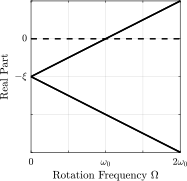
\includegraphics[width=\linewidth]{figs/campbell_diagram_real.pdf}
\caption{\label{fig:campbell_diagram_real} Real Part}
\end{subfigure}
\hfill
\begin{subfigure}[c]{0.4\linewidth}
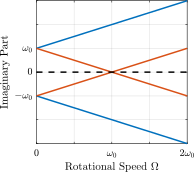
\includegraphics[width=\linewidth]{figs/campbell_diagram_imag.pdf}
\caption{\label{fig:campbell_diagram_imag} Imaginary Part}
\end{subfigure}
\hfill
\caption{\label{fig:campbell_diagram}Campbell Diagram : Evolution of the complex and real parts of the system's poles as a function of the rotational speed \(\Omega\)}
\centering
\end{figure}

Looking at the transfer function matrix \(\bm{G}_d\) in Eq. \eqref{eq:Gd_w0_xi_k}, one can see that the two diagonal (direct) terms are equal and the two off-diagonal (coupling) terms are opposite.
The bode plot of these two distinct terms are shown in Figure \ref{fig:plant_compare_rotating_speed} for several rotational speeds \(\Omega\).
These plots confirm the expected behavior: the frequency of the two pairs of complex conjugate poles are further separated as \(\Omega\) increases.
For \(\Omega > \omega_0\), the low frequency pair of complex conjugate poles \(p_{-}\) becomes unstable.

\begin{figure}[htbp]
\begin{subfigure}[c]{0.45\linewidth}
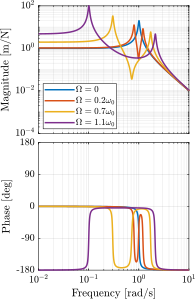
\includegraphics[width=\linewidth]{figs/plant_compare_rotating_speed_direct.pdf}
\caption{\label{fig:plant_compare_rotating_speed_direct} Direct Terms \(d_u/F_u\), \(d_v/F_v\)}
\end{subfigure}
\hfill
\begin{subfigure}[c]{0.45\linewidth}
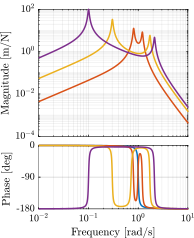
\includegraphics[width=\linewidth]{figs/plant_compare_rotating_speed_coupling.pdf}
\caption{\label{fig:plant_compare_rotating_speed_coupling} Coupling Terms \(d_v/F_u\), \(-d_u/F_v\)}
\end{subfigure}
\hfill
\caption{\label{fig:plant_compare_rotating_speed}Bode Plots for \(\bm{G}_d\) for several rotational speed \(\Omega\)}
\centering
\end{figure}

\section{Decentralized Integral Force Feedback}
\label{sec:org69e5bf1}
\label{sec:iff}
In order to apply IFF to the system, force sensors are added in series with the two actuators (Figure \ref{fig:system_iff}).
As this study focuses on decentralized control, two identical controllers \(K_F\) are used to feedback each of the sensed force to its associated actuator and no attempt is made to counteract the interactions in the system.
The control diagram is schematically shown in Figure \ref{fig:control_diagram_iff}.

\begin{minipage}[t]{0.50\linewidth}
\begin{center}
\includegraphics[width=\linewidth]{figs/system_iff.pdf}
\captionof{figure}{\label{fig:system_iff}System with added Force Sensor in series with the actuators}
\end{center}
\end{minipage}
\hfill
\begin{minipage}[t]{0.45\linewidth}
\begin{center}
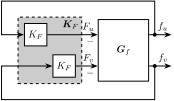
\includegraphics[width=\linewidth]{figs/control_diagram_iff.pdf}
\captionof{figure}{\label{fig:control_diagram_iff}Control Diagram for decentralized IFF}
\end{center}
\end{minipage}

\par
The forces \(\begin{bmatrix}f_u, f_v\end{bmatrix}\) measured by the two force sensors represented in Figure \ref{fig:system_iff} are equal to
\begin{equation}
\label{eq:measured_force}
  \begin{bmatrix} f_{u} \\ f_{v} \end{bmatrix} =
  \begin{bmatrix} F_u \\ F_v \end{bmatrix} - (c s + k)
  \begin{bmatrix} d_u \\ d_v \end{bmatrix}
\end{equation}

Inserting \eqref{eq:Gd_w0_xi_k} into \eqref{eq:measured_force} yields
\begin{equation}
\label{eq:Gf_mimo_tf}
  \begin{bmatrix} f_{u} \\ f_{v} \end{bmatrix} = \bm{G}_{f} \begin{bmatrix} F_u \\ F_v \end{bmatrix}
\end{equation}
with \(\bm{G}_f\) a \(2 \times 2\) transfer function matrix
\begin{equation}
\label{eq:Gf}
  \bm{G}_{f} = \begin{bmatrix}
  \frac{\left( \frac{s^2}{{\omega_0}^2} - \frac{\Omega^2}{{\omega_0}^2} \right) \left( \frac{s^2}{{\omega_0}^2} + 2 \xi \frac{s}{\omega_0} + 1 - \frac{{\Omega}^2}{{\omega_0}^2} \right) + \left( 2 \frac{\Omega}{\omega_0} \frac{s}{\omega_0} \right)^2}{\left( \frac{s^2}{{\omega_0}^2} + 2 \xi \frac{s}{\omega_0} + 1 - \frac{{\Omega}^2}{{\omega_0}^2} \right)^2 + \left( 2 \frac{\Omega}{\omega_0} \frac{s}{\omega_0} \right)^2} & \frac{- \left( 2 \xi \frac{s}{\omega_0} + 1 \right) \left( 2 \frac{\Omega}{\omega_0} \frac{s}{\omega_0} \right)}{\left( \frac{s^2}{{\omega_0}^2} + 2 \xi \frac{s}{\omega_0} + 1 - \frac{{\Omega}^2}{{\omega_0}^2} \right)^2 + \left( 2 \frac{\Omega}{\omega_0} \frac{s}{\omega_0} \right)^2} \\
  \frac{\left( 2 \xi \frac{s}{\omega_0} + 1 \right) \left( 2 \frac{\Omega}{\omega_0} \frac{s}{\omega_0} \right)}{\left( \frac{s^2}{{\omega_0}^2} + 2 \xi \frac{s}{\omega_0} + 1 - \frac{{\Omega}^2}{{\omega_0}^2} \right)^2 + \left( 2 \frac{\Omega}{\omega_0} \frac{s}{\omega_0} \right)^2} & \frac{\left( \frac{s^2}{{\omega_0}^2} - \frac{\Omega^2}{{\omega_0}^2} \right) \left( \frac{s^2}{{\omega_0}^2} + 2 \xi \frac{s}{\omega_0} + 1 - \frac{{\Omega}^2}{{\omega_0}^2} \right) + \left( 2 \frac{\Omega}{\omega_0} \frac{s}{\omega_0} \right)^2}{\left( \frac{s^2}{{\omega_0}^2} + 2 \xi \frac{s}{\omega_0} + 1 - \frac{{\Omega}^2}{{\omega_0}^2} \right)^2 + \left( 2 \frac{\Omega}{\omega_0} \frac{s}{\omega_0} \right)^2}
\end{bmatrix}
\end{equation}

The zeros of the diagonal terms of \(\bm{G}_f\) are equal to (neglecting the damping for simplicity)
\begin{subequations}
  \begin{align}
    z_c &= \pm j \omega_0 \sqrt{\frac{1}{2} \sqrt{8 \frac{\Omega^2}{{\omega_0}^2} + 1} + \frac{\Omega^2}{{\omega_0}^2} + \frac{1}{2} } \label{eq:iff_zero_cc} \\
    z_r &= \pm   \omega_0 \sqrt{\frac{1}{2} \sqrt{8 \frac{\Omega^2}{{\omega_0}^2} + 1} - \frac{\Omega^2}{{\omega_0}^2} - \frac{1}{2} } \label{eq:iff_zero_real}
  \end{align}
\end{subequations}

It can be easily shown that the frequency of the two complex conjugate zeros \(z_c\) \eqref{eq:iff_zero_cc} always lies between the frequency of the two pairs of complex conjugate poles \(p_{-}\) and \(p_{+}\) \eqref{eq:pole_values}.

For non-null rotational speeds, two real zeros \(z_r\) \eqref{eq:iff_zero_real} appear in the diagonal terms inducing a non-minimum phase behavior.
This can be seen in the Bode plot of the diagonal terms (Figure \ref{fig:plant_iff_compare_rotating_speed}) where the magnitude experiences an increase of its slope without any change of phase.

Similarly, the low frequency gain of \(\bm{G}_f\) is no longer zero and increases with the rotational speed \(\Omega\)
\begin{equation}
\label{low_freq_gain_iff_plan}
  \lim_{\omega \to 0} \left| \bm{G}_f (j\omega) \right| = \begin{bmatrix}
  \frac{\Omega^2}{{\omega_0}^2 - \Omega^2} & 0 \\
  0  & \frac{\Omega^2}{{\omega_0}^2 - \Omega^2}
\end{bmatrix}
\end{equation}

This low frequency gain can be explained as follows: a constant force \(F_u\) induces a small displacement of the mass \(d_u = \frac{F_u}{k - m\Omega^2}\), which increases the centrifugal force \(m\Omega^2d_u = \frac{\Omega^2}{{\omega_0}^2 - \Omega^2} F_u\) which is then measured by the force sensors.

\begin{figure}[htbp]
\centering
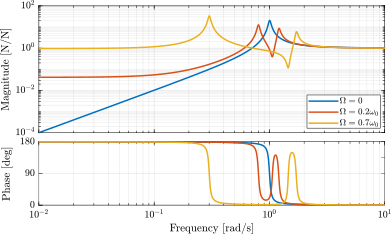
\includegraphics[scale=1]{figs/plant_iff_compare_rotating_speed.pdf}
\caption{\label{fig:plant_iff_compare_rotating_speed}Bode plot of the dynamics from a force actuator to its collocated force sensor (\(f_u/F_u\), \(f_v/F_v\)) for several rotational speeds \(\Omega\)}
\end{figure}

\par
\label{sec:iff_pure_int}
The two IFF controllers \(K_F\) consist of a pure integrator
\begin{equation}
\label{eq:Kf_pure_int}
  \bm{K}_F(s) = \begin{bmatrix} K_F(s) & 0 \\ 0 & K_F(s) \end{bmatrix}, \quad K_F(s) = g \cdot \frac{1}{s}
\end{equation}
where \(g\) is a scalar representing the gain of the controller.

In order to see how the IFF affects the poles of the closed loop system, a Root Locus (Figure \ref{fig:root_locus_pure_iff}) is constructed as follows: the poles of the closed-loop system are drawn in the complex plane as the gain \(g\) varies from \(0\) to \(\infty\) for the two controllers simultaneously.
As explained in \cite{preumont08_trans_zeros_struc_contr_with,skogestad07_multiv_feedb_contr}, the closed-loop poles start at the open-loop poles (shown by \(\tikz[baseline=-0.6ex] \node[cross out, draw=black, minimum size=1ex, line width=2pt, inner sep=0pt, outer sep=0pt] at (0, 0){};\)) for \(g = 0\) and coincide with the transmission zeros (shown by \(\tikz[baseline=-0.6ex] \draw[line width=2pt, inner sep=0pt, outer sep=0pt] (0,0) circle[radius=3pt];\)) as \(g \to \infty\).
The direction of increasing gain is indicated by arrows \(\tikz[baseline=-0.6ex] \draw[-{Stealth[round]},line width=2pt] (0,0) -- (0.3,0);\).

\begin{figure}[htbp]
\centering
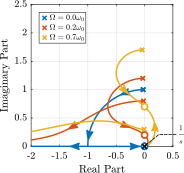
\includegraphics[scale=1]{figs/root_locus_pure_iff.pdf}
\caption{\label{fig:root_locus_pure_iff}Root Locus for the decentralized IFF: evolution of the closed-loop poles with increasing gains. This is done for several rotating speeds \(\Omega\)}
\end{figure}

Whereas collocated IFF is usually associated with unconditional stability \cite{preumont91_activ}, this property is lost as soon as the rotational speed in non-null due to gyroscopic effects.
This can be seen in the Root Locus (Figure \ref{fig:root_locus_pure_iff}) where the pole corresponding to the controller is bound to the right half plane implying closed-loop system instability.

Physically, this can be explained by realizing that below some frequency, the loop gain being very large, the decentralized IFF effectively decouples the payload from the XY stage.
Moreover, the payload experiences centrifugal forces, which can be modeled by negative stiffnesses pulling it away from the rotation axis rendering the system unstable, hence the poles in the right half plane.

In order to apply Decentralized IFF on rotating positioning stages, two solutions are proposed to deal with this instability problem.
The first one consists of slightly modifying the control law (Section \ref{sec:iff_hpf}) while the second one consists of adding springs in parallel with the force sensors (Section \ref{sec:iff_kp}).

\section{Integral Force Feedback with High Pass Filter}
\label{sec:orgaa5d9a8}
\label{sec:iff_hpf}
As was explained in the previous section, the instability when using IFF with pure integrators comes from high controller gain at low frequency.

In order to limit the low frequency controller gain, an high pass filter (HPF) can be added to the controller
\begin{equation}
\label{eq:IFF_LHF}
  \bm{K}_F(s) = \begin{bmatrix} K_F(s) & 0 \\ 0 & K_F(s) \end{bmatrix}, \quad K_{F}(s) = g \cdot \frac{1}{s} \cdot \underbrace{\frac{s/\omega_i}{1 + s/\omega_i}}_{\text{HPF}} = g \cdot \frac{1}{s + \omega_i}
\end{equation}

This is equivalent to slightly shifting the controller pole to the left along the real axis.

This modification of the IFF controller is typically done to avoid saturation associated with the pure integrator \cite{preumont91_activ}.
This is however not the case in this study as it will become clear in the next section.

\par
The loop gains for the decentralized controllers \(K_F(s)\) with and without the added HPF are shown in Figure \ref{fig:loop_gain_modified_iff}.
The effect of the added HPF limits the low frequency gain as expected.

The Root Loci for the decentralized IFF with and without the HPF are displayed in Figure \ref{fig:root_locus_modified_iff}.
With the added HPF, the poles of the closed loop system are shown to be stable up to some value of the gain \(g_\text{max}\)
\begin{equation}
\label{eq:gmax_iff_hpf}
  g_{\text{max}} = \omega_i \left( \frac{{\omega_0}^2}{\Omega^2} - 1 \right)
\end{equation}
It is interesting to note that \(g_{\text{max}}\) also corresponds to the gain where the low frequency loop gain (Figure \ref{fig:loop_gain_modified_iff}) reaches one.

\begin{minipage}[b]{0.45\linewidth}
\begin{center}
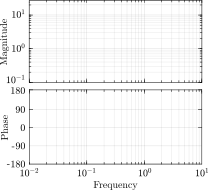
\includegraphics[scale=1]{figs/loop_gain_modified_iff.pdf}
\captionof{figure}{\label{fig:loop_gain_modified_iff}Modification of the loop gain with the added HFP, \(g = 2\), \(\omega_i = 0.1 \omega_0\) and \(\Omega = 0.1 \omega_0\)}
\end{center}
\end{minipage}
\hfill
\begin{minipage}[b]{0.5\linewidth}
\begin{center}
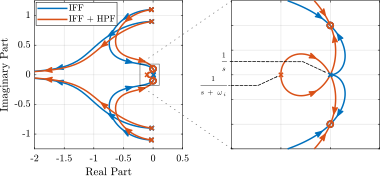
\includegraphics[scale=1]{figs/root_locus_modified_iff.pdf}
\captionof{figure}{\label{fig:root_locus_modified_iff}Modification of the Root Locus with the added HPF, \(\omega_i = 0.1 \omega_0\) and \(\Omega = 0.1 \omega_0\)}
\end{center}
\end{minipage}

\par
Two parameters can be tuned for the controller \eqref{eq:IFF_LHF}: the gain \(g\) and the pole's location \(\omega_i\).
The optimal values of \(\omega_i\) and \(g\) are here considered as the values for which the damping of all the closed-loop poles are simultaneously maximized.

In order to visualize how \(\omega_i\) does affect the attainable damping, the Root Loci for several \(\omega_i\) are displayed in Figure \ref{fig:root_locus_wi_modified_iff}.
It is shown that even though small \(\omega_i\) seem to allow more damping to be added to the system resonances, the control gain \(g\) may be limited to small values due to Eq. \eqref{eq:gmax_iff_hpf}.

\begin{figure}[htbp]
\centering
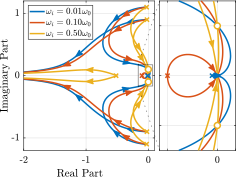
\includegraphics[scale=1]{figs/root_locus_wi_modified_iff.pdf}
\caption{\label{fig:root_locus_wi_modified_iff}Root Locus for several HPF cut-off frequencies \(\omega_i\), \(\Omega = 0.1 \omega_0\)}
\end{figure}

In order to study this trade off, the attainable closed-loop damping ratio \(\xi_{\text{cl}}\) is computed as a function of the ratio \(\omega_i/\omega_0\).
The gain \(g_{\text{opt}}\) at which this maximum damping is obtained is also display and compared with the gain \(g_{\text{max}}\) at which the system becomes unstable (Figure \ref{fig:mod_iff_damping_wi}).

Three regions can be observed:
\begin{itemize}
\item \(\frac{\omega_i}{\omega_0} < 0.02\): the added damping is limited by the maximum allowed control gain \(g_{\text{max}}\)
\item \(0.02 < \frac{\omega_i}{\omega_0} < 0.2\): good amount of damping can be added for \(g \approx 2\)
\item \(0.2 < \frac{\omega_i}{\omega_0}\): the added damping becomes small due to the shape of the Root Locus (Figure \ref{fig:root_locus_wi_modified_iff})
\end{itemize}

\begin{figure}[htbp]
\centering
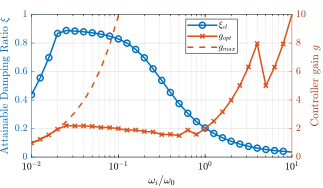
\includegraphics[scale=1]{figs/mod_iff_damping_wi.pdf}
\caption{\label{fig:mod_iff_damping_wi}Attainable damping ratio \(\xi_\text{cl}\) as a function of the ratio \(\omega_i/\omega_0\). Corresponding control gain \(g_\text{opt}\) and \(g_\text{max}\) are also shown}
\end{figure}

\section{Integral Force Feedback with Parallel Springs}
\label{sec:orge64ac7f}
\label{sec:iff_kp}
As was explained in section \ref{sec:iff_pure_int}, the instability when using decentralized IFF for rotating positioning platforms is due to Gyroscopic effects and, more precisely, due to the negative stiffness induced by centrifugal forces.
In this section additional springs in parallel with the force sensors are added to counteract this negative stiffness.
Such springs are schematically shown in Figure \ref{fig:system_parallel_springs} where \(k_a\) is the stiffness of the actuator and \(k_p\) the stiffness in parallel with the actuator and force sensor.

Amplified piezoelectric stack actuators can also be used for such purpose where a part of the piezoelectric stack is used as an actuator while the rest is used as a force sensor \cite{souleille18_concep_activ_mount_space_applic}.
The parallel stiffness \(k_p\) then corresponds to the amplification structure.
An example of such system is shown in Figure \ref{fig:cedrat_xy25xs}.

\begin{minipage}[t]{0.48\linewidth}
\begin{center}
\includegraphics[width=\linewidth]{figs/system_parallel_springs.pdf}
\captionof{figure}{\label{fig:system_parallel_springs}Studied system with additional springs in parallel with the actuators and force sensors}
\end{center}
\end{minipage}
\hfill
\begin{minipage}[t]{0.48\linewidth}
\begin{center}
\includegraphics[width=\linewidth]{figs/cedrat_xy25xs.png}
\captionof{figure}{\label{fig:cedrat_xy25xs}XY Piezoelectric Stage (XY25XS from Cedrat Technology)}
\end{center}
\end{minipage}

\par
The forces \(\begin{bmatrix}f_u, f_v\end{bmatrix}\) measured by the two force sensors represented in Figure \ref{fig:system_parallel_springs} are equal to
\begin{equation}
\label{eq:measured_force_kp}
  \begin{bmatrix} f_{u} \\ f_{v} \end{bmatrix} =
  \begin{bmatrix} F_u \\ F_v \end{bmatrix} - (c s + k_a)
  \begin{bmatrix} d_u \\ d_v \end{bmatrix}
\end{equation}

In order to keep the overall stiffness \(k = k_a + k_p\) constant, a scalar parameter \(\alpha\) (\(0 \le \alpha < 1\)) is defined to describe the fraction of the total stiffness in parallel with the actuator and force sensor
\begin{equation}
  k_p = \alpha k, \quad k_a = (1 - \alpha) k
\end{equation}

The equations of motion are derived and transformed in the Laplace domain
\begin{equation}
\label{eq:Gk_mimo_tf}
\begin{bmatrix} f_u \\ f_v \end{bmatrix} =
\bm{G}_k
\begin{bmatrix} F_u \\ F_v \end{bmatrix}
\end{equation}
with \(\bm{G}_k\) a \(2 \times 2\) transfer function matrix
\begin{equation}
\label{eq:Gk}
\bm{G}_k =
\begin{bmatrix}
  \frac{\left( \frac{s^2}{{\omega_0}^2} - \frac{\Omega^2}{{\omega_0}^2} + \alpha \right) \left( \frac{s^2}{{\omega_0}^2} + 2 \xi \frac{s}{\omega_0} + 1 - \frac{{\Omega}^2}{{\omega_0}^2} \right) + \left( 2 \frac{\Omega}{\omega_0} \frac{s}{\omega_0} \right)^2}{\left( \frac{s^2}{{\omega_0}^2} + 2 \xi \frac{s}{\omega_0} + 1 - \frac{{\Omega}^2}{{\omega_0}^2} \right)^2 + \left( 2 \frac{\Omega}{\omega_0} \frac{s}{\omega_0} \right)^2} & \frac{- \left( 2 \xi \frac{s}{\omega_0} + 1 - \alpha \right) \left( 2 \frac{\Omega}{\omega_0} \frac{s}{\omega_0} \right)}{\left( \frac{s^2}{{\omega_0}^2} + 2 \xi \frac{s}{\omega_0} + 1 - \frac{{\Omega}^2}{{\omega_0}^2} \right)^2 + \left( 2 \frac{\Omega}{\omega_0} \frac{s}{\omega_0} \right)^2} \\
  \frac{\left( 2 \xi \frac{s}{\omega_0} + 1 - \alpha \right) \left( 2 \frac{\Omega}{\omega_0} \frac{s}{\omega_0} \right)}{\left( \frac{s^2}{{\omega_0}^2} + 2 \xi \frac{s}{\omega_0} + 1 - \frac{{\Omega}^2}{{\omega_0}^2} \right)^2 + \left( 2 \frac{\Omega}{\omega_0} \frac{s}{\omega_0} \right)^2} & \frac{\left( \frac{s^2}{{\omega_0}^2} - \frac{\Omega^2}{{\omega_0}^2} + \alpha \right) \left( \frac{s^2}{{\omega_0}^2} + 2 \xi \frac{s}{\omega_0} + 1 - \frac{{\Omega}^2}{{\omega_0}^2} \right) + \left( 2 \frac{\Omega}{\omega_0} \frac{s}{\omega_0} \right)^2}{\left( \frac{s^2}{{\omega_0}^2} + 2 \xi \frac{s}{\omega_0} + 1 - \frac{{\Omega}^2}{{\omega_0}^2} \right)^2 + \left( 2 \frac{\Omega}{\omega_0} \frac{s}{\omega_0} \right)^2}
\end{bmatrix}
\end{equation}

Comparing \(\bm{G}_k\) \eqref{eq:Gk} with \(\bm{G}_f\) \eqref{eq:Gf} shows that while the poles of the system are kept the same, the zeros of the diagonal terms have changed.
The two real zeros \(z_r\) \eqref{eq:iff_zero_real} that were inducing non-minimum phase behavior are transformed into complex conjugate zeros if the following condition hold
\begin{equation}
\label{eq:kp_cond_cc_zeros}
  \alpha > \frac{\Omega^2}{{\omega_0}^2} \quad \Leftrightarrow \quad k_p > m \Omega^2
\end{equation}

Thus, if the added parallel stiffness \(k_p\) is higher than the negative stiffness induced by centrifugal forces \(m \Omega^2\), the direct dynamics from actuator to force sensor will show minimum phase behavior.
This is confirmed by the Bode plot in Figure \ref{fig:plant_iff_kp}.

Figure \ref{fig:root_locus_iff_kp} shows Root Loci plots for \(k_p = 0\), \(k_p < m \Omega^2\) and \(k_p > m \Omega^2\) when \(K_F\) is a pure integrator \eqref{eq:Kf_pure_int}.
It is shown that if the added stiffness is higher than the maximum negative stiffness, the poles of the closed-loop system stay in the (stable) right half-plane, and hence the unconditional stability of IFF is recovered.

\begin{minipage}[b]{0.42\linewidth}
\begin{center}
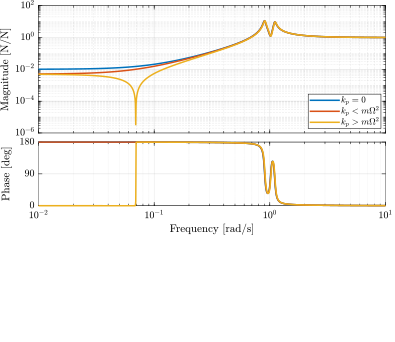
\includegraphics[scale=1]{figs/plant_iff_kp.pdf}
\captionof{figure}{\label{fig:plant_iff_kp}Bode Plot of \(f_u/F_u\) without parallel spring, with parallel springs with stiffness \(k_p < m \Omega^2\) and \(k_p > m \Omega^2\), \(\Omega = 0.1 \omega_0\)}
\end{center}
\end{minipage}
\hfill
\begin{minipage}[b]{0.52\linewidth}
\begin{center}
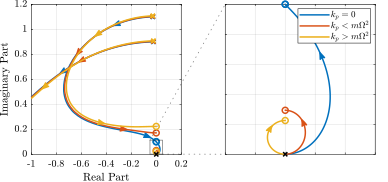
\includegraphics[scale=1]{figs/root_locus_iff_kp.pdf}
\captionof{figure}{\label{fig:root_locus_iff_kp}Root Locus for IFF without parallel spring, with parallel springs with stiffness \(k_p < m \Omega^2\) and \(k_p > m \Omega^2\), \(\Omega = 0.1 \omega_0\)}
\end{center}
\end{minipage}

\par
Even though the parallel stiffness \(k_p\) has no impact on the open-loop poles (as the overall stiffness \(k\) stays constant), it has a large impact on the transmission zeros.
Moreover, as the attainable damping is generally proportional to the distance between poles and zeros \cite{preumont18_vibrat_contr_activ_struc_fourt_edition}, the parallel stiffness \(k_p\) is foreseen to have a large impact on the attainable damping.

To study this effect, Root Locus plots for several parallel stiffnesses \(k_p > m \Omega^2\) are shown in Figure \ref{fig:root_locus_iff_kps}.
The frequencies of the transmission zeros of the system are increasing with the parallel stiffness \(k_p\) and the associated attainable damping is reduced.
Therefore, even though the parallel stiffness \(k_p\) should be larger than \(m \Omega^2\) for stability reasons, it should not be taken too high as this would limit the attainable bandwidth.

For any \(k_p > m \Omega^2\), the control gain \(g\) can be tuned such that the maximum simultaneous damping \(\xi_\text{opt}\) is added to the resonances of the system.
An example is shown in Figure \ref{fig:root_locus_opt_gain_iff_kp} for \(k_p = 5 m \Omega^2\) where the damping \(\xi_{\text{opt}} \approx 0.83\) is obtained for a control gain \(g_\text{opt} \approx 2 \omega_0\).

\begin{figure}[htbp]
\begin{subfigure}[c]{0.45\linewidth}
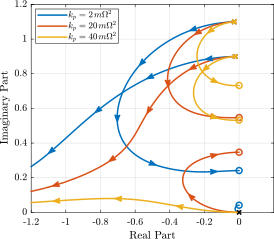
\includegraphics[width=\linewidth]{figs/root_locus_iff_kps.pdf}
\caption{\label{fig:root_locus_iff_kps} Comparison of three parallel stiffnesses \(k_p\)}
\end{subfigure}
\hfill
\begin{subfigure}[c]{0.45\linewidth}
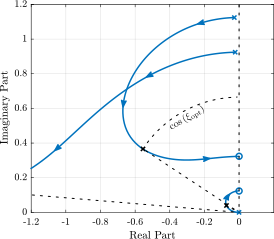
\includegraphics[width=\linewidth]{figs/root_locus_opt_gain_iff_kp.pdf}
\caption{\label{fig:root_locus_opt_gain_iff_kp} \(k_p = 5 m \Omega^2\), optimal damping \(\xi_\text{opt}\) is shown}
\end{subfigure}
\hfill
\caption{\label{fig:root_locus_iff_kps_opt}Root Locus for IFF when parallel stiffness \(k_p\) is added, \(\Omega = 0.1 \omega_0\)}
\centering
\end{figure}

\section{Comparison and Discussion}
\label{sec:org118e3e9}
\label{sec:comparison}
Two modifications to the decentralized IFF for rotating positioning stages have been proposed.

The first modification concerns the controller and consists of adding an high pass filter to \(K_F\) \eqref{eq:IFF_LHF}.
The system was shown to be stable for gains up to \(g_\text{max}\) \eqref{eq:gmax_iff_hpf}.

The second proposed modification concerns the mechanical system.
It was shown that if springs with a stiffness \(k_p > m \Omega^2\) are added in parallel to the actuators and force sensors, decentralized IFF can be applied with unconditional stability.

These two methods are now compared in terms of added damping, closed-loop compliance and transmissibility.
For the following comparisons, the cut-off frequency for the high pass filters is set to \(\omega_i = 0.1 \omega_0\) and the parallel springs have a stiffness \(k_p = 5 m \Omega^2\).

\par
Figure \ref{fig:comp_root_locus} shows two Root Locus plots for the two proposed IFF techniques.
While the two pairs of complex conjugate open-loop poles are identical for both techniques, the transmission zeros are not.
This means that their closed-loop behavior will differ when large control gains are used.

It is interesting to note that the maximum added damping is very similar for both techniques and is reached for the same control gain in both cases \(g_\text{opt} \approx 2 \omega_0\).

\begin{figure}[htbp]
\centering
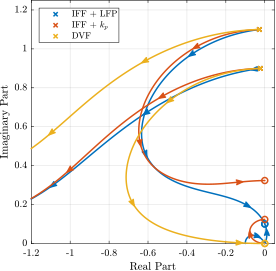
\includegraphics[scale=1]{figs/comp_root_locus.pdf}
\caption{\label{fig:comp_root_locus}Root Locus for the two proposed modifications of decentralized IFF, \(\Omega = 0.1 \omega_0\)}
\end{figure}

\par
The two proposed techniques are now compared in terms of closed-loop compliance and transmissibility.

The compliance is defined as the transfer function from external forces applied to the payload to the displacement of the payload in an inertial frame.
The transmissibility describes the dynamic behaviour between the displacement of the rotating stage and the displacement of the payload.
It is used to characterize how much vibration of the rotating stage is transmitted to the payload.

The two techniques are also compared with passive damping (Figure \ref{fig:system}) where \(c = c_\text{crit}\) is tuned to critically damp the resonance when the rotating speed is null.

\begin{equation}
  c_\text{crit} = 2 \sqrt{k m}
\end{equation}

Very similar results are obtained for the two proposed decentralized IFF modifications in terms of compliance (Figure \ref{fig:comp_compliance}) and transmissibility (Figure \ref{fig:comp_transmissibility}).
It is also confirmed that these two techniques can significantly damp the system's resonances.

Compared to passive damping, the two techniques degrade the compliance at low frequency (Figure \ref{fig:comp_compliance}).
They however do not degrade the transmissibility at high frequency as it is the case with passive damping (Figure \ref{fig:comp_transmissibility}).

\begin{figure}[htbp]
\begin{subfigure}[c]{0.45\linewidth}
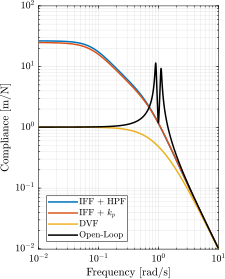
\includegraphics[width=\linewidth]{figs/comp_compliance.pdf}
\caption{\label{fig:comp_compliance} Compliance}
\end{subfigure}
\hfill
\begin{subfigure}[c]{0.45\linewidth}
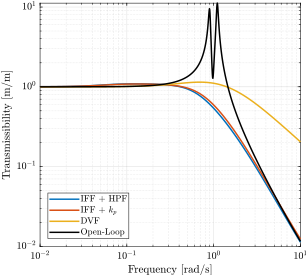
\includegraphics[width=\linewidth]{figs/comp_transmissibility.pdf}
\caption{\label{fig:comp_transmissibility} Transmissibility}
\end{subfigure}
\hfill
\caption{\label{fig:comp_active_damping}Comparison of the two proposed Active Damping Techniques, \(\Omega = 0.1 \omega_0\)}
\centering
\end{figure}

\section{Conclusion}
\label{sec:org419f838}
\label{sec:conclusion}




\section*{Acknowledgment}
\label{sec:org19e4dbd}
This research benefited from a FRIA grant from the French Community of Belgium.

\bibliography{ref.bib}
\end{document}
